\subsection{Enunciado del problema}
\textbf{Minimizando el número de visitas al proveedor:}\\

Un granjero necesita disponer siempre de un determinado fertilizante. La cantidad máxima que puede almacenar la consume en r días, y antes de que eso ocurra necesita acudir a una tienda del pueblo para abastecerse. El problema es que dicha tienda tiene un horario de apertura muy irregular (solo abre determinados días). El granjero conoce los días en que abre la tienda, y desea minimizar el número de desplazamientos al pueblo para abastecerse.\\

\begin{itemize}
\item Diseñar un algoritmo greedy que determine en qué días debe acudir al pueblo a comprar fertilizante durante un periodo de tiempo determinado (por ejemplo durante el siguiente mes).\\
\item Demostrar que el algoritmo encuentra siempre la solución  óptima.\\
\end{itemize}


\subsection{Diseño del algoritmo}

El algoritmo, al basarse en la filosofía greedy, intenta escoger la mejor solución en cada fase. En nuestro caso, la mejor solución pasa por ir a comprar el día más lejano posible que cumpla estas dos condiciones.\\
\begin{enumerate}
\item Que diste menos de r días de la ultima reposición.\\
\item Que la tienda esté abierta.\\
\end{enumerate}

\textbf{Ejemplo:} \hyperref[ejemplo]{(Figura 1)}\\
\begin{figure}[h]
\centering
	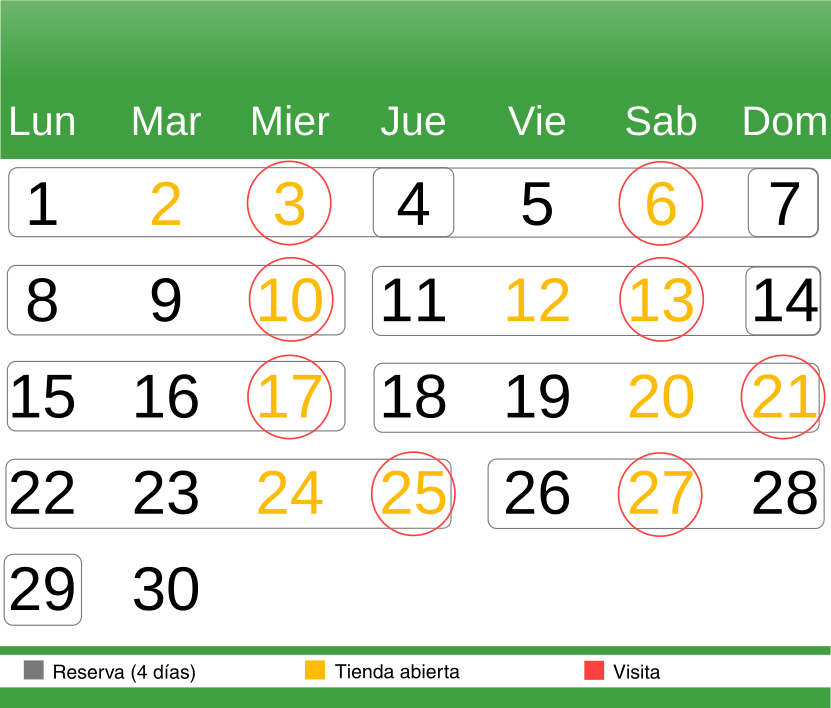
\includegraphics[width=1\textwidth]{Imagenes/calendario.png}
	\caption{Ejemplo} 
\end{figure}
\label{ejemplo} 


\subsubsection{Representación del algoritmo}

Para programar el problema lo hemos modelado de la siguiente manera:\\

\begin{itemize}
\item Un vector de booleanos representa los días que abre la tienda.\\
Por ejemplo [1, 0, 0, 1, 0, 1] significa que la tienda abre los días 1, 4 y 6.\\
\item Una lista de enteros almacena los días que el granjero tiene que ir a comprar.
\end{itemize}


\subsubsection{Implementación del algoritmo}

La implementación se encuentra en \textit{minimizar\_visitas.cpp}.\\
La función clave es \textbf{minimize\_visits()}, en la que, para buscar el día mas lejano posible, se accede a la posición i+r del vector y se recorre hacia atrás hasta que se encuentra un día en el que la tienda esté abierta.\\

También hemos implementado otro algoritmo con el fin de hacer comparaciones, en el que el día de visita se elige aleatoriamente en el rango [i, i+r-1]. Esta implementación se encuentra en \textit{visitas\_aleatorias.cpp}\\



\subsection{Demostración de la optimalidad}
